\section{瞬态响应和稳态响应分析}
\subsection{瞬态响应和稳态响应}
\begin{itemize}
	\item	瞬态响应:系统从初始状态到最终状态的响应过程
	\item	稳态响应:系统在时间$t$趋于无穷大时的系统输出状态
\end{itemize}

系统响应可表示为
\begin{equation*}
c(t)=c_{tr}(t)+c_{ss}(t)
\end{equation*}

其中,$c_{tr}(t)$为瞬态响应(transient),$c_{ss}(t)$为稳态响应(steady-state)。

\subsection{灵敏度传递函数}

\begin{figure}[!ht]
	\centering
	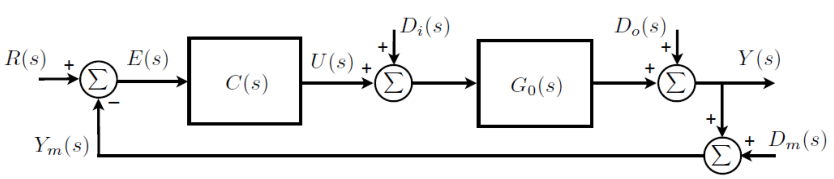
\includegraphics[width=\linewidth]{figures/34.png}
	\caption{典型的反馈控制系统}
	\label{34}
\end{figure}

图\ref{34}所示的是一个典型的反馈控制系统,其中$R(s)$为输入信号,$Y(s)$为输出信号,$U(s)$为控制信号,$D_i(s)$, $D_o(s)$, $D_m(s)$分别为被控对象的输入、输出误差与与测量误差。

\begin{align*}
	G_0(s)&=\frac{B_0(s)}{A_0(s)}\quad&\mbox{$B_0(s), A_0(s)$互质}\\
	C(s)&=\frac{P(s)}{L(s)}\quad&\mbox{$P(s), Ls)$互质}\\ 
	\Lambda_0(s)&=C(s)G_0(s)
\end{align*}

由此我们可以得到四个灵敏度传递函数:

\begin{itemize}
	\item Complementary Sensitivity
	
	\begin{equation*}
		T_{0}(s)=\frac{\Lambda_{0}(s)}{1+\Lambda_{0}(s)}
	\end{equation*}

	\item (Output) Sensitivity
	
	\begin{equation*}
		S_{0}(s)=\frac{1}{1+\Lambda_{0}(s)}
	\end{equation*}

	\item Input-disturbance Sensitivity
	
	\begin{equation*}
		S_{i 0}(s)=\frac{G_{0}(s)}{1+\Lambda_{0}(s)}
	\end{equation*}

	\item Control Sensitivity
	
	\begin{equation*}
		S_{u 0}(s)=\frac{C(s)}{1+\Lambda_{0}(s)}
	\end{equation*}
\end{itemize}

从而有

\begin{align*}
	Y(s)=T_{0}(s) R(s)+S_{0}(s) D_{o}(s)+S_{i 0} D_{i}(s)-T_{0}(s) D_{m}(s)\\ 
	U(s)=S_{u 0}(s)\left(R(s)-D_{m}(s)-D_{o}(s)-G_{0}(s) D_{i}(s)\right)
\end{align*}

\subsection{一阶系统}

\begin{figure}[!ht]
	\centering
	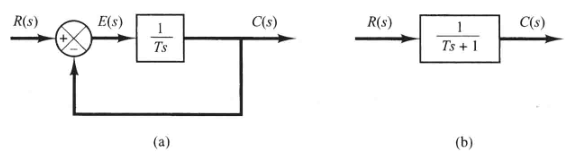
\includegraphics[width=12cm]{figures/5.png}
	\caption{一阶系统}
	\label{5}
\end{figure}

如图\ref{5},一阶系统的传递函数为

\begin{equation*}
G(s)=\frac{C(s)}{R(s)}=\frac{1}{1+Ts}
\end{equation*}

\subsubsection{单位阶跃响应}

单位阶跃响应的拉普拉斯变换为$1/s$,代入得到

\begin{equation*}
C(s)=\frac{1}{1+Ts}\frac{1}{s}=\frac{1}{s}-\frac{1}{s+\frac1T}
\end{equation*}

对上式作拉普拉斯反变换,有

\begin{equation*}
c(T)=\Laplace^{-1}C(s)=1-e^{-{t}/{T}}
\end{equation*}

\begin{figure}[!ht]
	\centering
	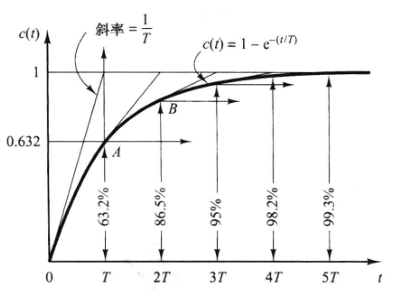
\includegraphics[width=8cm]{figures/6.png}
	\caption{一阶系统阶跃响应}
	\label{6}
\end{figure}

对应的时间常数$T$越小,系统的响应就越快。由图\ref{6}可以看出,当$t\ge4T$时,响应的误差将保持在2\%以内。$4T$可以作为响应时间的估值。

\subsubsection{单位斜坡响应}

单位斜坡函数的拉普拉斯变换为$1/s^2$,对应的输出可以表达为
\begin{gather*}
C(s)=\frac{1}{1+Ts}\frac{1}{s^2}=\frac{1}{s^2}-\frac{T}{s}+\frac{T^2}{1+Ts}\\
C(t)=\Laplace^{-1}[C(s)]=t-T+Te^{-t/T}
\end{gather*}

误差信号$e(t)$则为

\begin{gather*}
e(t)=r(t)-c(t)=T(1-e^{-t/T})\\
e(\infty)=T
\end{gather*}

\begin{figure}[!ht]
	\centering
	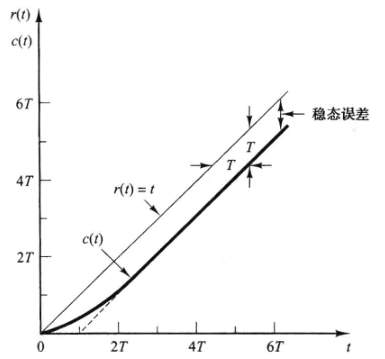
\includegraphics[width=8cm]{figures/7.png}
	\caption{一阶系统斜坡响应}
	\label{7}
\end{figure}

如图\ref{7},对于单位斜坡输入,其响应存在稳态误差$T$,因此时间常数越小,其稳态误差越小。

\subsubsection{单位脉冲响应}

单位脉冲输入信号可表示为狄拉克函数$\delta(t)$(其本质为泛函),其拉普拉斯变换为$R(s)=1$。系统的输出等于

\begin{gather*}
C(s)=\frac{1}{1+Ts}\\
c(t)=\Laplace^{-1}[C(s)]=\frac{1}{T}e^{-t/T}
\end{gather*}

\begin{figure}[!ht]
	\centering
	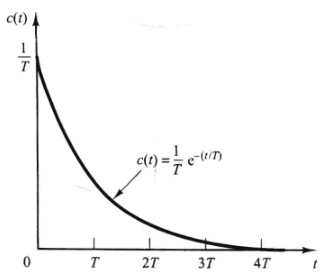
\includegraphics[width=8cm]{figures/8.png}
	\caption{一阶系统脉冲响应}
	\label{8}
\end{figure}

其响应曲线如图\ref{8}所示。

\subsubsection{线性定常系统特性}

对于线性定常系统,其输入信号求导,则输出信号也求导;其输入信号积分,其输出也积分。这是线性定常系统独有的特性,线性时变系统和非线性系统不具备这种特性。

\subsection{二阶系统}

\begin{figure}[!ht]
	\centering
	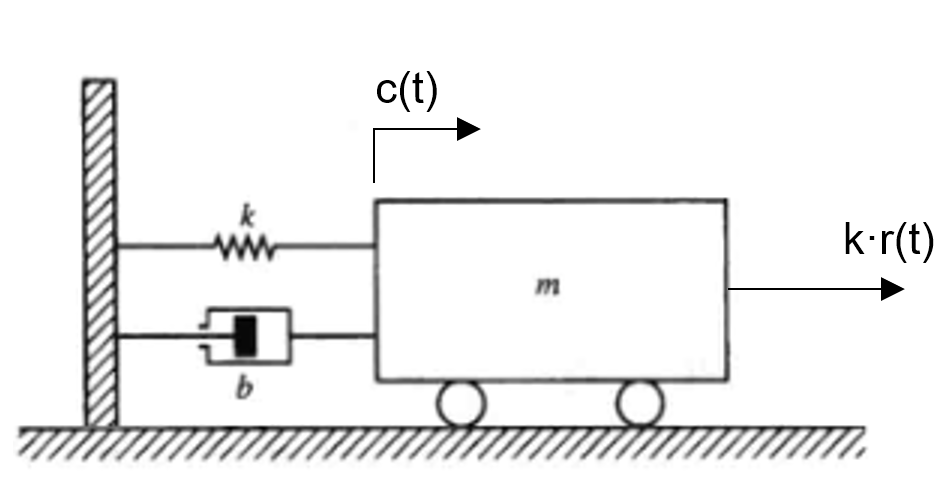
\includegraphics[width=8cm]{figures/9.png}
	\caption{二阶振动系统}
	\label{9}
\end{figure}

如图\ref{9}所示的振动系统,可以容易地列写出对应的微分方程与传递函数:

\begin{gather*}
m\ddot c+b\dot c+kc=kr(t)\\
(ms^2+bs+k)C(s)=kR(s)\\
\frac{C(s)}{R(s)}=\frac{k}{ms^2+bs+k}=\frac{k/m}{s^2+\frac{b}{m}s+\frac{k}{m}}
\end{gather*}

不难看出,传递函数具有两个极点,故此称为二阶系统。

可以将传递函数再改写为

\begin{equation*}
\frac{C(s)}{R(s)}=\frac{\frac{k}{m}}{\left[s+\frac{b}{2m}+\sqrt{(\frac{b}{m})^2-\frac{4k}{m}}\right]\left[s+\frac{b}{2m}-\sqrt{(\frac{b}{m})^2-\frac{4k}{m}}\right]}
\end{equation*}

当$b^2-2mk<0$时,闭环极点为共轭复数;当$b^2-2mk\ge0$时,闭环极点为实数。引入参量:

\begin{align*}
\omega_n^2&:=\frac{k}{m}\\
\sigma&:=\frac{b}{2m}=\zeta\omega_n
\end{align*}

式中,$\sigma$为衰减系数,$\omega_n$为无阻尼自然频率,$\zeta$为系统阻尼比。$\zeta$同时也是实际阻尼系数$b$与临界阻尼系数$b_c=2\sqrt{mk}$的比值。

传递函数可以改写成这样的形式:

\begin{equation*}
\frac{C(s)}{R(s)}=\frac{\omega_n^2}{s^2+2\zeta\omega_ns+\omega_n^2}
\end{equation*}

$\zeta=0$时,瞬态响应的振荡将永不停止;$0<\zeta<1$时,闭环极点为共轭复数,系统欠阻尼,响应会是振荡的;$\zeta=1$时,系统为临界阻尼系统;$\zeta>1$时,系统为过阻尼系统。

\subsubsection{单位阶跃响应}

对于单位阶跃信号的输入,其拉普拉斯变换为$R(s)=1/s$,对应的响应为

\begin{equation*}
C(s)=\frac{\omega_n^2}{(s^2+2\zeta\omega_ns+\omega_n^2)s}
\end{equation*}

\begin{enumerate}
	\item	欠阻尼情况($0<\zeta<1$)

	定义阻尼自然频率$\omega_d=\omega_n\sqrt{1-\zeta^2}$,则

	\begin{align*}
	C(s)&=\frac{\omega_n^2}{(s^2+2\zeta\omega_ns+\omega_n^2)s}\\
	&=\frac1s-\frac{s+2\zeta\omega_n}{(s^2+2\zeta\omega_ns+\omega_n^2)}\\
	&=\frac1s-\frac{s+\zeta\omega_n}{(s^2+2\zeta\omega_ns+\omega_n^2)}-\frac{\zeta\omega_n}{(s^2+2\zeta\omega_ns+\omega_n^2)}
	\end{align*}

	等式两边做拉普拉斯反变换,则有

	\begin{align*}
	c(t)&=\Laplace^{-1}[C(s)]\\
	&=1-e^{-\zeta\omega_nt}\cos\omega_dt-e^{-\zeta\omega_nt}\frac{\zeta}{\sqrt{1-\zeta^2}}\sin\omega_dt\\
	&=1-\frac{e^{-\zeta\omega_nt}}{\sqrt{1-\zeta^2}}\sin\left(\omega_dt+\arctan\frac{\sqrt{1-\zeta^2}}{\zeta}\right)
	\end{align*}

	可以看出,稳态时误差为$0$,瞬态振荡频率为阻尼自然频率$\omega_d$,它由无阻尼自然频率$\omega_n$和阻尼比$\zeta$决定。

	将$\zeta=0$代入,可以得到无阻尼振荡的响应

	\begin{equation*}
	c(t)=1-\cos\omega_nt
	\end{equation*}
	
	为无限期振荡。

	\item	临界阻尼情况($\zeta=1$)

	若两个极点相等,此时构成临界阻尼系统,

	\begin{gather*}
	C(s)=\frac{\omega_n^2}{(s+\omega_n)^2s}\\
	c(t)=1-e^{\omega_nt}(1+\omega_nt)
	\end{gather*}

	\item	过阻尼情况($\zeta>1$)

	此时极点为两个不等的负实数。

	\begin{align*}
	C(s)&=\frac{\omega_n^2}{\left(s+\zeta\omega_n+\omega_n\sqrt{\zeta^2-1}\right)\left(s+\zeta\omega_n-\omega_n\sqrt{\zeta^2-1}\right)}\\
	c(t)&=1+\frac{1}{2\sqrt{\zeta^2-1}\left(\zeta+\sqrt{\zeta^2-1}\right)}e^{-\left(\zeta+\sqrt{\zeta^2-1}\right)\omega_nt}\\
	&\hspace{2em}-\frac{1}{2\sqrt{\zeta^2-1}\left(\zeta-\sqrt{\zeta^2-1}\right)}e^{-\left(\zeta-\sqrt{\zeta^2-1}\right)\omega_nt}\\
	&=1+\frac{\omega_n}{2\sqrt{\zeta^2-1}}\left(\frac{e^{-s_1t}}{s_1}-\frac{e^{-s_2t}}{s_2}\right)
	\end{align*}

	式中,$s_1=\left(\zeta+\sqrt{\zeta^2-1}\right)\omega_n$,$s_2=\left(\zeta-\sqrt{\zeta^2-1}\right)\omega_n$。这是两个衰减的指数项。在$\zeta>>1$时,即阻尼极大,衰减项的影响将主要取决于衰减较慢的那一项;也就是说,当$\left|{s_2}\right|<<\left|{s_1}\right|$时,可以忽略$s_1$的影响。在这样的前提下,传递函数可近似表示为

	\begin{equation*}
	\frac{C(s)}{R(s)}=\frac{s_2}{s+s_2}
	\end{equation*}

	其单位阶跃响应为

	\begin{align*}
	C(s)&=\frac{s_2}{\left(s+s_2\right)s}\\
	c(t)&=1-e^{-\left(\zeta-\sqrt{\zeta^2-1}\right)\omega_nt}
	\end{align*}

\end{enumerate}

\begin{figure}[!ht]
	\centering
	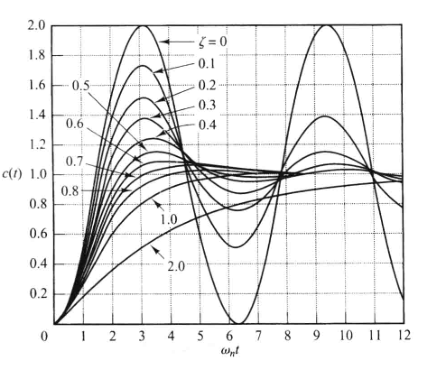
\includegraphics[width=8cm]{figures/10.png}
	\caption{不同阻尼比的单位阶跃响应曲线}
	\label{10}
\end{figure}

\subsubsection{瞬态响应指标}

对于单位阶跃输入信号的瞬态响应特性,用下列性能指标衡量,如图\ref{11}:

\begin{enumerate}
	\item	延迟时间$t_d$:响应曲线第一次达到稳态值一般所需的时间。
	\item	上升时间$t_r$:响应曲线从稳态值的10\%上升至90\%所需的时间,或是5\%上升至90\%,或是0\%上升至100\%所需的时间。
	\item	峰值时间$t_p$:响应曲线达到过调量的第一个峰值所需要的时间。
	\item	最大过调量$M_p$:从$1$开始计算的响应曲线的最大峰值为最大过调量。若响应稳态值不为$1$,则采用最大百分比过调量:
	\begin{equation*}
	\mbox{最大百分比过调量}=\frac{c(t_p)-c(\infty)}{c(\infty)}\times100\%
	\end{equation*}
	\item	调整时间$t_s$:响应曲线的稳态线上,稳态值的上下$2\%$或$5\%$以内作为允许误差范围;响应曲线达到并且永远处于这一误差范围内所需的时间即为调整时间。	
\end{enumerate}

\begin{figure}[!ht]
	\centering
	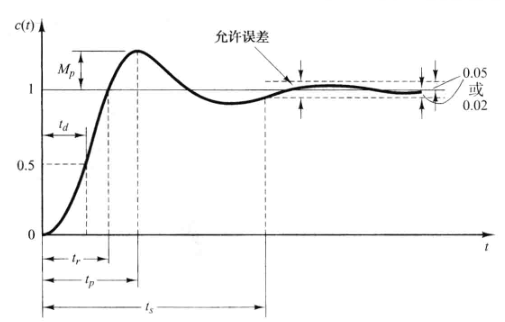
\includegraphics[width=8cm]{figures/11.png}
	\caption{单位阶跃响应的性能指标}
	\label{11}
\end{figure}

为了获得比较好的二阶系统瞬态响应特性,阻尼比必须选择在$0.4\sim0.8$之间。阻尼比过小会造成严重过调,而过大的阻尼比则会使系统响应变得缓慢。另一方面,最大过调量和上升时间存在Trade off关系,无法兼得。

\subsubsection{二阶系统的瞬态响应指标}

假设系统为欠阻尼二阶系统

\begin{enumerate}
	\item	上升时间$t_r$
	令$c(t_r)=1$,可得

	\begin{equation*}
	t_r=\frac{1}{\omega_d}\arctan\left(\frac{\omega_d}{-\sigma}\right)=\frac{\pi-\beta}{\omega_d}
	\end{equation*}

	其中$\beta$角的定义如图\ref{12}所示。

	\begin{figure}[!ht]
		\centering
		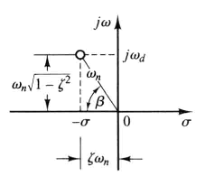
\includegraphics[width=8cm]{figures/12.png}
		\caption{$\beta$角的定义}
		\label{12}
	\end{figure}

	\item	峰值时间$t_p$
	令$dc(t)/dt=0$,可得

	\begin{align*}
	\sin\omega_dt_p=0\\
	t_p=\frac{\pi}{\omega_d}
	\end{align*}

	\item	最大过调量$M_p$

	最大过调量在峰值时间取到,直接代入$t_p$:

	\begin{align*}
	M_p&=c(t_p)-1\\
	&=e^{-(\sigma/\omega_d)\pi}\\
	&=e^{-(\zeta/\sqrt{1-\zeta^2})\pi}
	\end{align*}

	\item	调整时间$t_s$

	\begin{align*}
	t_s=4T=\frac{4}{\sigma}=\frac{4}{\zeta\omega_n}\hspace{2mm}\mbox{2\%误差标准}\\
	t_s=3T=\frac{3}{\sigma}=\frac{3}{\zeta\omega_n}\hspace{2mm}\mbox{5\%误差标准}
	\end{align*}
	
\end{enumerate}

经验公式:

对于二阶系统,要求$\delta=0.01y_\infty$时,有

\begin{equation*}
	\sigma\geq\frac{4.6}{t_s}
\end{equation*}

$\sigma$为极点距虚轴距离

定义$t_r$为$0.1y_\infty\rightarrow0.9y_\infty$,

\begin{equation*}
	\omega_n\geq\frac{1.8}{t_r}
\end{equation*}

$\omega_n$为极点距原点距离

给定最大过调量$M_p$,

\begin{equation*}
	\zeta\geq\frac{-\frac{\ln M_p}{\pi}}{\sqrt{1+\frac{\ln^2M_p}{\pi^2}}}
\end{equation*}

由图\ref{12}可知,$\cos\beta=\zeta,\quad\beta=\arccos\zeta$

\subsubsection{单位脉冲响应}

对于脉冲响应$r(t)=\delta(t)$,其拉普拉斯变换为$R(s)=1$,因此

\begin{align*}
C(s)&=\frac{\omega_n^2}{s^2+2\zeta\omega_ns+\omega_n^2}\\
c(t)&=\Laplace^{-1}[C(s)]
\end{align*}

\begin{enumerate}
	\item	$0\le\zeta<1$
	\begin{equation*}
	c(t)=\frac{\omega_n}{\sqrt{1-\zeta^2}}e^{-\zeta\omega_nt}\sin\omega_n\sqrt{1-\zeta^2}t
	\end{equation*}
	
	\item	$\zeta=1$
	\begin{equation*}
	c(t)=\omega_n^2te^{-\omega_nt}
	\end{equation*}

	\item	$\zeta>1$
	\begin{equation*}
	c(t)=\frac{\omega_n}{2\sqrt{\zeta^2-1}}e^{-(\zeta-\sqrt{\zeta^2-1})\omega_nt}-\frac{\omega_n}{2\sqrt{\zeta^2-1}}e^{-(\zeta+\sqrt{\zeta^2-1})\omega_nt}
	\end{equation*}
\end{enumerate}

对于临界阻尼和过阻尼的情况,单位脉冲响应总是非负的,$c(t)\ge0$。



\subsection{高阶系统}

对于高阶系统而言,往往考虑其主导极点(距离虚轴最近的一对共轭极点),二阶系统所给出的规律仍然具有指导意义。换言之,可以根据系统要求的瞬态响应指标,在复平面上给出``允许极点存在的位置''。事实上在处理高阶系统时,系统的频域响应更加重要。

\subsection{劳斯稳定判据}

劳斯稳定判据的作用是,对一个关于$s$的多项式方程,在无需实际求解这一方程,就可以判断系统的绝对稳定性。

多项式方程:

\begin{equation*}
a_0s^n+a_1s^{n-1}+\cdots+a_{n-1}s+a_n=0
\end{equation*}

其中$a_n\neq0$,即不存在零根。

\begin{itemize}
	\item	确保所有系数都是正的(如果全是负的则乘以$-1$到方程两边)。如果有负系数,则方程一定存在正根,即存在右半平面的极点,系统不稳定。
	\item	将多项式排列成下列形式:

	\begin{tabular}{llllll}
	$s^n$	&$a_0$	&$a_2$	&$a_4$	&$a_6$	& $\cdots$	\\
	$s^{n-1}$	&$a_1$	&$a_2$	&$a_3$	&$a_4$	& $\cdots$	\\
	$s^{n-2}$	&$b_1$	&$b_2$	&$b_3$	&$b_4$	& $\cdots$	\\
	$s^{n-3}$	&$c_1$	&$c_2$	&$c_3$	&$c_4$	& $\cdots$	\\
	$s^{n-4}$	&$d_1$	&$d_2$	&$d_3$	&$d_4$	& $\cdots$	\\
	$\vdots$	&$\vdots$	&$\vdots$\\
	$s^{2}$	&$e_1$	&$e_2$\\
	$s^{1}$	&$f_1$\\
	$s^{0}$	&$g_1$
	\end{tabular}

	其中,$b$,$c$,$d$,$e$等系数为

	\begin{equation*}
	\frac{\mbox{左下}\times\mbox{右上}-\mbox{左上}\times\mbox{右下}}{\mbox{左下}}
	\end{equation*}
	
	即

	\begin{align*}
	b_1&=\frac{a_1a_2-a_0a_3}{a_1}\\
	b_2&=\frac{a_1a_4-a_0a_5}{a_1}\\
	b_2&=\frac{a_1a_6-a_0a_7}{a_1}\\
	&\vdots\\
	c_1&=\frac{b_1a_3-a_1b_2}{b_1}\\
	c_2&=\frac{b_1a_5-a_1b_3}{b_1}\\
	c_3&=\frac{b_1a_7-a_1b_4}{b_1}\\
	&\vdots\\
	d_1&=\frac{c_1b_2-b_1c_2}{c_1}\\
	d_2&=\frac{c_1b_3-b_1c_3}{c_1}\\
	&\vdots
	\end{align*}
	
	直到用完所有行(没有数的地方视为$0$)。
\end{itemize}

劳斯稳定判据指出,多项式方程中,实部大于$0$的根数(右半平面极点),等于劳斯阵列中第一列系数符号的改变次数。所以,方程所有根在左半平面的充要条件是,劳斯阵列第一列所有项均为正数。

\begin{enumerate}
	\item	可以在列写劳斯阵列的过程中,把某一行整体乘以或除以一个正数,简化计算。
	\item	如果某一行的第一项等于零,但其余各项不等于零或没有其余项,则可以用一个很小的正数$\epsilon$代替该项。如果$\epsilon$上下的符号一致,则表明有一对纯虚根存在;若上下符号相反,则意味着一次变号。
	\item	如果某一行全为0,则意味着存在大小相等但互为相反数的一对根。这时,可以将最后一行非零行对应的系数构成一个辅助多项式,对该多项式求导,把求导后的系数作为新的行。
\end{enumerate}

\subsection{单位反馈控制系统中的稳态误差}

\subsubsection{控制系统分类}

开环传递函数

\begin{equation*}
G(s)=\frac{K(T_as+1)(T_bs+1)\cdots(T_ms+1)}{s^N(T_1s+1)(T_2s+1)\cdots(T_ps+1)}
\end{equation*}

$G(s)$分母中$s^N$项表示它在原点处有$N$重极点,称系统为$N$型系统(有别于$n$阶系统)。类型号数增加,系统精度会得到改善,但稳定性会随之下降。

\subsubsection{稳态误差}

由于开环传递函数为$G(s)$,且反馈为单位反馈,则闭环传递函数

\begin{equation*}
\frac{C(s)}{R(s)}=\frac{G(s)}{1+G(s)}
\end{equation*}

误差信号为

\begin{align*}
E(s)&=\frac{1}{1+G(s)}R(s)\\
e_{ss}&=\lim_{t\to\infty}e(t)=\lim_{s\to0}sE(s)=\lim_{s\to0}\frac{sR(s)}{1+G(s)}
\end{align*}

稳态误差小结:

\begin{center}
	\begin{tabular}{|c|c|c|c|}
			\hline
				&	阶跃输入$r(t)=1$	&	斜坡输入$r(t)=t$	&	加速度输入$r(t)=\frac12t^2$\\\hline
			0型系统&	$\frac{1}{1+K}$	&$\infty$	&	$\infty$\\\hline
			1型系统&$0$	&$\frac1K$&$\infty$\\\hline
			2型系统&$0$	&$0$	&$\frac1K$\\\hline
	\end{tabular}
\end{center}






